\subsection{Registration}
We can now look at how our similarity measures perform when we make a rigid and affine registration. In the simplest case we can make a rigid self registration (image A with image A) using NMI. Because we know an optimal transformation matrix will have $\theta = 0$, $t_x = 0$ and $t_y = 0$ we can initialize the transformation matrix to have $\theta = 0.2$, $t_x = 5$ and $t_y = 5$ and see if it returns to all zeros. If we let our gradient descend optimizer run for 200 iterations with a rotation learning rate of 1 and a translation learning rate of 100 we get that the final transformation matrix have $\theta =  0.0023$, $t_x = -0.039$ and $t_y = -0.014$ which is very close to our expectation.\\
We can now perform a rigid transformation using NMI again, but this time using image A and B. We begin by initializing $\theta = 0.3$, $t_x = 5$ and $t_y = 5$. The results can be seen in \autoref{rigidNMIAB}.

\begin{figure}[h]
	\centering
	\begin{subfigure}{0.4\linewidth}
		\centering
		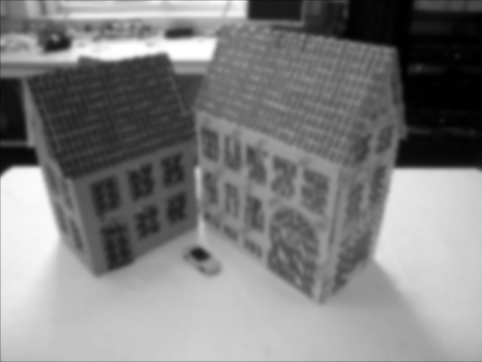
\includegraphics[width=\linewidth]{Materials/rigidNMIAB}
		\caption{Transformed image.\newline}
	\end{subfigure}
	\hspace{1cm}
	\begin{subfigure}{0.4\linewidth}
		\centering
		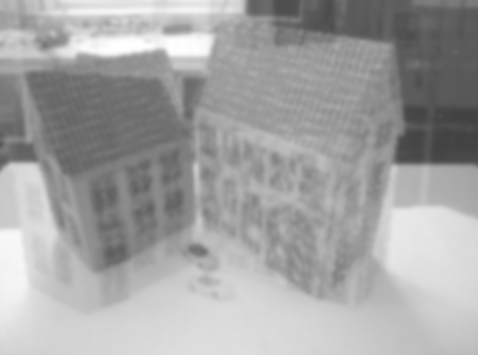
\includegraphics[width=\linewidth]{Materials/rigidNMIABO}
		\caption{Target image overlaid with transformed image.}
	\end{subfigure}
	\caption{Result of rigid registration using NMI on image A and B.}
	\label{rigidNMIAB}
\end{figure}
\begin{figure}
	\centering
	\begin{subfigure}{0.4\linewidth}
		\centering
		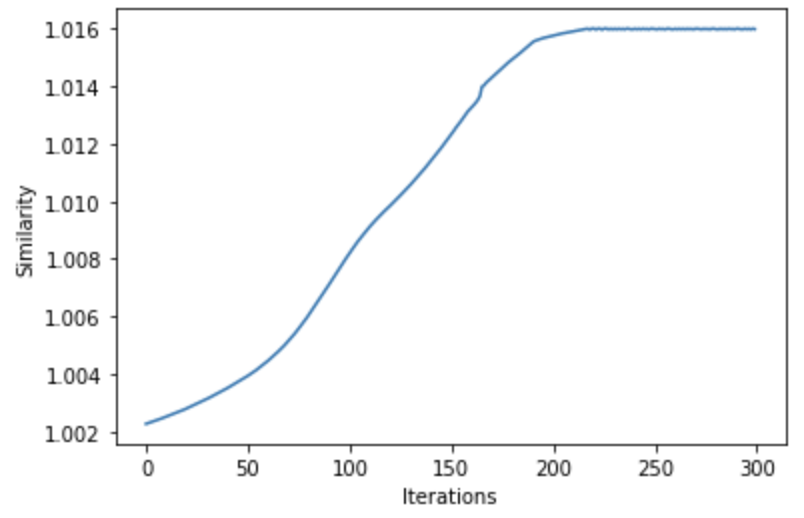
\includegraphics[width=\linewidth]{Materials/RigidNMILoss}
		\caption{Similarity using NMI at each iteration of optimization with translation learning rate of 100 and rotation learning rate at 1.}
		\label{rigidNMIABLoss}
	\end{subfigure}
	\hspace{1cm}
	\begin{subfigure}{0.4\linewidth}
		\centering
		\includegraphics[width=\linewidth]{Materials/RigidNCCLoss}
		\caption{Similarity using NCC at each iteration of optimization with translation learning rate of 10 and rotation learning rate at 0.1.}
		\label{rigidNCCABLoss}
	\end{subfigure}

\end{figure}
We see that the optimized transformation matrix goes towards 0 for all parameters which means it finds the optimal transformation to be no transformation. This is also consistent with the results seen in the object similarity section. In \autoref{rigidNMIABLoss} we see the similarity at each iteration of the optimization, and we see we have found an optima. As discussed earlier, the reason for the optimal parameters being 0 are probably because the foreground is dominant in the images, and optimizing the amount of foreground is probably better than optimizing the overlap of buildings.\\
We can now perform a rigid registration using NCC, image A and image B inverted. Here we initialize with the same parameters, but use a rotation learning rate of 0.1 and a translation learning rate of 10. The results can be seen in \autoref{rigidNCCAB}, and the similarity at each iteration can be seen in \autoref{rigidNCCABLoss}.

\begin{figure}[h]
	\centering
	\begin{subfigure}{0.4\linewidth}
		\centering
		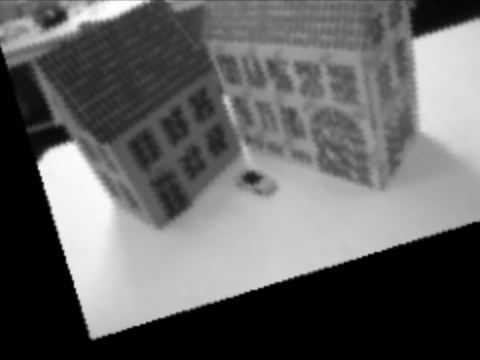
\includegraphics[width=\linewidth]{Materials/rigidNCCAB}
		\caption{Transformed image.\newline}
	\end{subfigure}
	\hspace{1cm}
	\begin{subfigure}{0.4\linewidth}
		\centering
		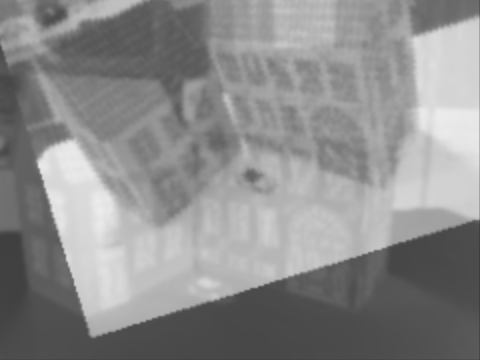
\includegraphics[width=\linewidth]{Materials/rigidNCCABO}
		\caption{Target image overlaid with transformed image.}
	\end{subfigure}
	\caption{Result of rigid registration using NCC on image A and inverted B.}
	\label{rigidNCCAB}
\end{figure}
We here note the motif is getting turned out of the resulting image. This is likely again because the foreground is attempted matched, and rotating the image introduces black pixels into the foreground. This illustrates that NCC is \textit{not} intensity invariant. We also note from \autoref{rigidNCCABLoss} that we have not yet reached an optima, which means if we ran more iterations or used bigger learning rates, the image would get further rotate.\\
We can now perform an affine registration using NMI and image A and B. We initialize the transformation matrix with the same $\theta$, $t_x$ and $t_y$ values as before and initialize $s_x = s_y = 1.2$. The rotation learning rate is set to 0.7, for translation it set to 100, and for scaling it is set to 1. The results can be seen in \autoref{affineNMIAB} and the similarity at each iteration can be seen in \autoref{affineNMIABLoss}.

\begin{figure}[h]
	\centering
	\begin{subfigure}{0.4\linewidth}
		\centering
		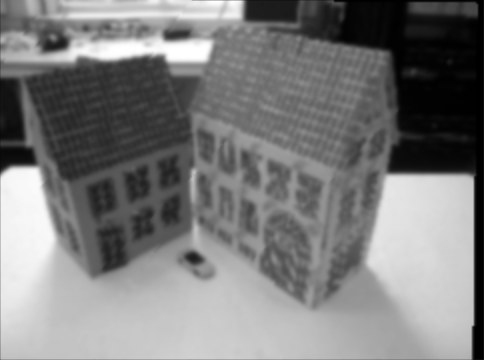
\includegraphics[width=\linewidth]{Materials/affineNMIAB}
		\caption{Transformed image.\newline}
	\end{subfigure}
	\hspace{1cm}
	\begin{subfigure}{0.4\linewidth}
		\centering
		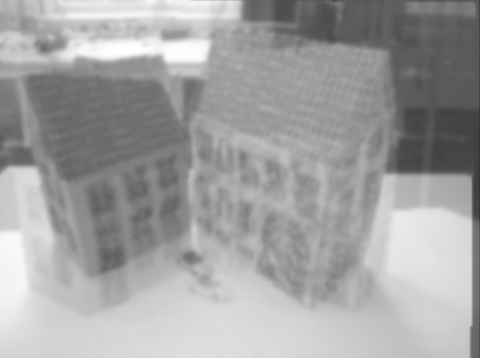
\includegraphics[width=\linewidth]{Materials/affineNMIABO}
		\caption{Target image overlaid with transformed image.}
	\end{subfigure}
	\caption{Result of affine registration using NMI on image A and B.}
	\label{affineNMIAB}
\end{figure}
\begin{figure}[h]
	\centering
	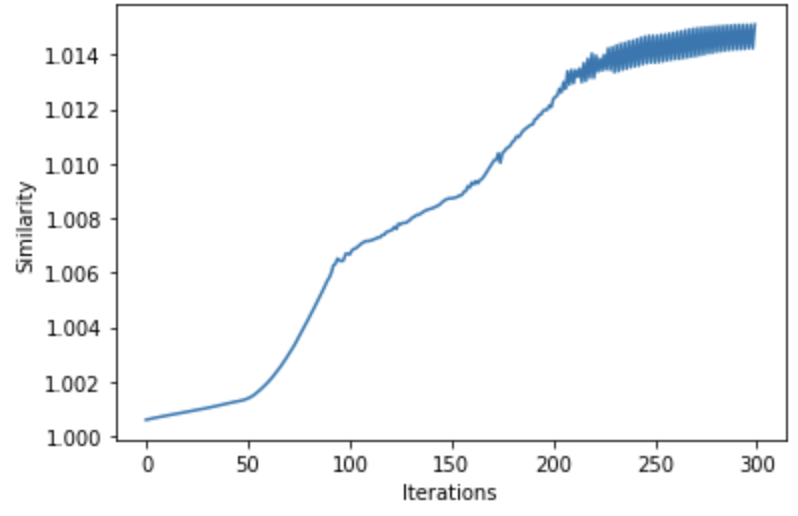
\includegraphics[width=0.4\linewidth]{Materials/affineNMIABLoss}
	\caption{Similarity at each iteration for affine registration between image A and B using NMI.}
	\label{affineNMIABLoss}
\end{figure}
We here note it is attempted to align the foreground of the images, however looking at \autoref{affineNMIABLoss} we see some volatile oscillation towards the end indicating we are using too big learning rates. This is likely the reason the the transformation matrix is not returning to 0 displacement. However, we see the houses and the car overlap slightly more than before. 